\documentclass{article}

\setlength{\parindent}{0pt}
\usepackage{graphicx}
\usepackage{hyperref}
\usepackage{amsmath}

\graphicspath{{../images/}}

\begin{document}

\section{H-3.1}

The dispersive channel can introduce inter-symbol interference.
This can lead to more bit errors.
Thus the bit error curves for the dispersive channel are shifted to the right of the bit error curves for the AWGN channel, as the error increases for the same SNR.

\section{H-3.2}

One can calculate the delay spread of the channel by measuring the time between the first and last peaks of the impulse response.
Alternatively, one can measure the (coherence?) bandwidth and take the reciprocal.

\section{H-3.3}

\begin{figure}[h]
\centering
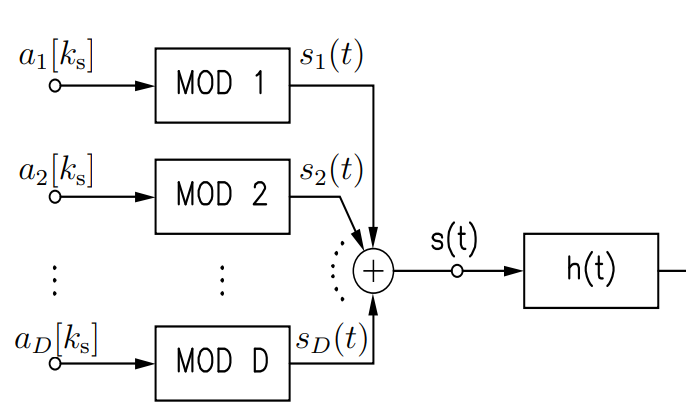
\includegraphics[width=0.6\textwidth]{ofdm_transmitter.png}
\caption{OFDM transmitter}
\label{fig:ofdm_transmitter}
\end{figure}

\section{H-3.4}

The amount of samples need to be as long as the multipath channel length.
So devide the multipath channel length by the length of one sample to get the amount of samples needed.

\section{H-3.5}

\begin{figure}[h]
\centering
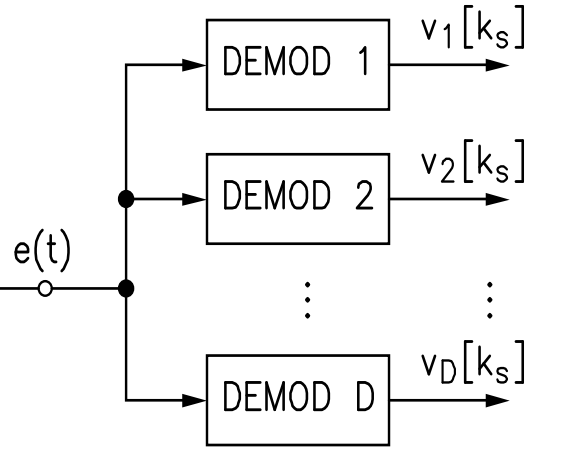
\includegraphics[width=0.6\textwidth]{ofdm_receiver.png}
\caption{OFDM receiver}
\label{fig:ofdm_receiver}
\end{figure}


\section{H-3.6}
Yes, its possible that there are no errors when the channels get combined again by the FEQ function.

\end{document}
